The previous section perfectly segues into this section. \textit{Cross products} is an operation on vectors that happens solely in the third dimension. Do not confuse it with the dot product, both uses different operators and should not be used interchangeably. Firstly, we must recall that one of the basis vectors is \(\khat\) and it is one unit in the z direction.
\begin{marginfigure}
  \centering
  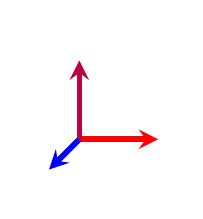
\begin{tikzpicture}
    \draw[line width=2pt, -stealth, red] (0,0,0) -- (1,0,0) node[pos=1.1]{\(\ihat\)};
    \draw[line width=2pt, -stealth, blue] (0,0,0) -- (0,0,1) node[pos=1.4]{\(\jhat\)};
    \draw[line width=2pt, -stealth, purple] (0,0,0) -- (0,1,0) node[pos=1.3]{\(\khat\)};
  \end{tikzpicture}
  \caption{Figure of the three basis vectors.}
\end{marginfigure}
